\documentclass[12pt]{article}
\usepackage[margin=48pt]{geometry}
\usepackage{amsthm}
\usepackage{parskip}
\usepackage{graphicx}
\usepackage{enumerate}
\usepackage{subfigure}
\usepackage[usenames]{color}


\renewcommand{\thesection}{\Roman{section}} 
\renewcommand{\thesubsection}{\thesection.\Roman{subsection}}


\begin{document}

\thispagestyle{empty}
\begin{figure}[h!]
\centering

\includegraphics[width=2in]{epfl.pdf}
\vspace{1em}
\end{figure}
\hrule
\vspace{1em}
\begin{center}
{\Huge Second Practical} \\
\vspace{1.5em}
Castellon, Joel. Murgia, Matteo.
\end{center}
\vspace{1.5em}
\hrule

\vspace{1.5em}

\begin{center}
{\Large \bf Summary}
\end{center}
We analyze a small car dataset issued from consumer reports in the U.S. We start
with a Gaussian linear model and asses our assumptions with two criteria: statistical
significance and symptoms of multicollinearity.
Our goal is two-fold: first is to build more complex models from our initial setup. Then we 
study the properties of automatic procedures for model selection (Forward selection, Backward elimination).

We find that in our problem (\emph{cars} dataset) there is a fundamental trade-off between significance
and variance inflation. While it is not clear on how to generalize this issue to get further insight, we have
found enormous value in the interplay of automatic procedures and exploratory analysis stemming from
the experience of the researcher.
Indeed, no procedure or criterion for model selection is free of assumptions nor is the analyst.
But this process facilitates the research for associations in both parties.

\vspace{1em}

\tableofcontents

\vfill

\hrule

\newpage
\setcounter{page}{1}
\section{Introduction}
In this practical we explore model selection procedures in the cars dataset.
We have two main questions. First, we explore the difference when
we vary the order in which variables enter the model in the ANOVA procedure for:
\begin{equation}\label{eq:model}
\frac{100}{City MPG} = \beta_0 + \beta_1Weight + \beta_2\frac{Horsepower}{Weight} + \epsilon
\end{equation}
Because in this first question our model is very simple (2 covariates), ANOVA's
F statistic is sufficient as we can only have one nested model each time.

Second, we aim to build a more complex model using covariates in the range $\{11 \ldots 26\}$.
For this purpose we use \emph{Forward Selection} and \emph{Backwards Elimination} both
with AIC and BIC criteria. To asses the models obtained we look at the presence of multicollinearity on these. For this purpose we use the Variance Inflation Factor \emph{VIF}
because it provides a measure of how much each covariate is explained by the rest of the model.

We also elaborate on our results with some exploratory analysis on the
scatter plots between covariates in the second group. Both Forward/Backwards procedures as AIC and BIC have different properties, we thus
obtain alternative results. We elaborate this discussion in the \emph{Analysis} section.

\section{The data} \label{sec:thedata}
The data comes from the April 1993 issue of U.S consumer reports.
We briefly point out why a linear model is a reasonable fit, a detailed
exploratory analysis was done First Practical. Here we present the parts
that will serve to asses and elaborate on the model selection procedures we employ.

Indeed, if we plot the output variable \texttt{Gallons per hundred city miles} against both \texttt{Weight} and \texttt{Pure power}(Horsepower/Weight) (Figure \ref{fig:scatter}).

\begin{figure}[h]
\centering
\subfigure[Output Variable vs PurePower\label{subfig:ScatterPower}]{
	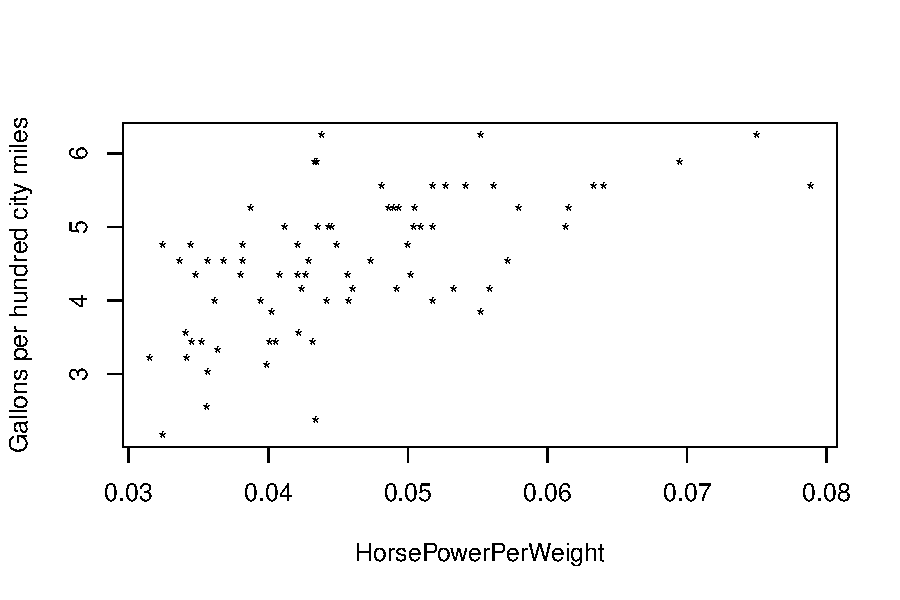
\includegraphics[width=3in]{ScatterPower.pdf}
}
\subfigure[Output Variable vs Weights\label{subfig:ScatterWeights}]{
	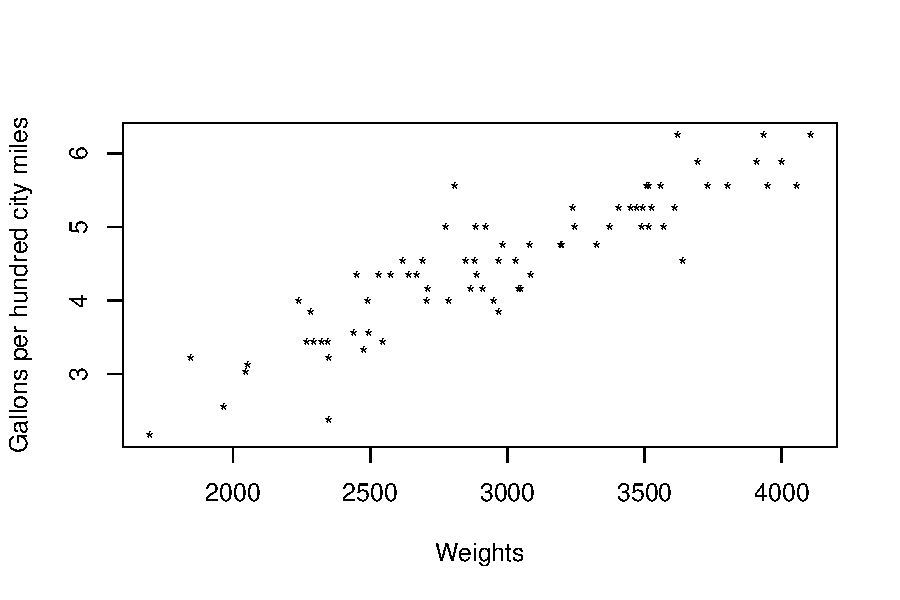
\includegraphics[width=3in]{ScatterWeights.pdf}
}
\caption{Scatter plots of covariates against output variable.}
\label{fig:scatter}
\end{figure}

We see the output variable has a clear linear dependence with the \texttt{Weight} covariate and less so with the \texttt{Pure power} (Correlation coefficient 0.900 and 0.597 respectively).
This observation will be relevant when explaining ANOVA results for our first question.

For our second question we present the main dependencies in the second group of covariates $\{11\ldots 26\}$ (Figure \ref{fig:pairs}).
This will be will be relevant when we take out some variables from the second group and run
again our model selection procedures.
\begin{figure}[h!]
\centering
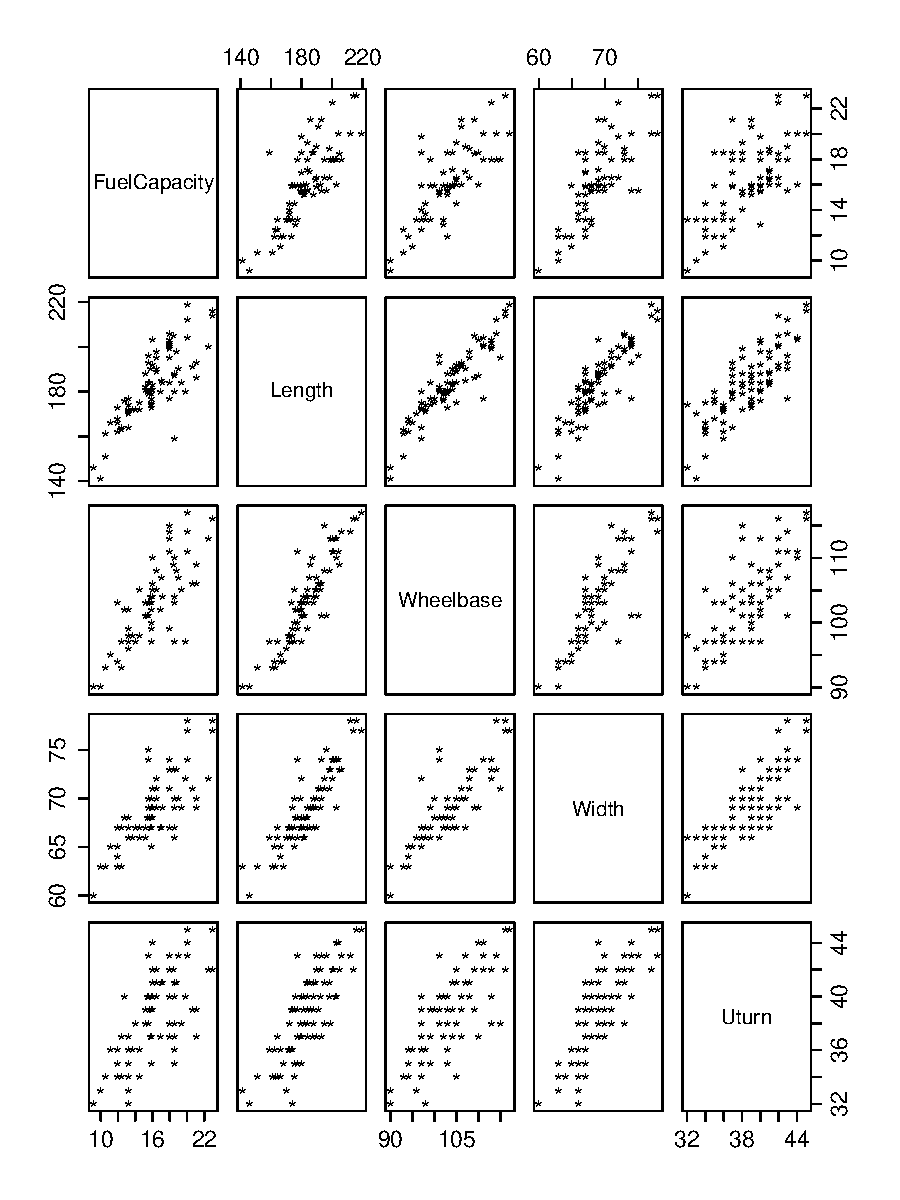
\includegraphics[width=6in,height=8in]{Pairs.pdf}
\caption{Pair scatter plots between covariates in the group \{11 to 26\} that we will consider to remove because of their dependencies.}
\label{fig:pairs}
\end{figure}

\section{Methodology}\label{sec:themethod}
Our main tools in this study are ANOVA, Forward Selection, Backwards Elimintion and 
the AIC/BIC criteria.
\subsection{ANOVA}
The Analysis of Variance (ANOVA) is a procedure for building submodels from a pool of
explanatory variables (\texttt{anova} function in \cite{R}). The procedure starts with the intercept and ads one variable
at the time. At each step the significance in the reduction of the Residual Sum of Squares (RSS) is measured (from the previous model). Then we know whether the variable 
we want to add to the model really increases the explanatory capacity of the model. It is clear, from simple experimentation that on the average case the order in which we enter the variables \emph{does matter}. So, we
might build several different models.
More details can be found in chapter 15 of \cite{ARA}.

\subsection{Forward Selection and Backward Elimination}
Both forward selection and backwards elimination are greedy algorithms, in the sense
that they choose the \emph{best} candidate at each iteration. Forward selection starts
with the intercept and always select the variable (group of variables if we are more general) that has the most significant reduction in RSS. In our case, we complement by
using the AIC/BIC criteria (\texttt{step} function in \cite{R}) which would be the minimum for such \emph{best} candidate. This algorithm stops when no covariate (or term) can be added such that the reduction in RSS is significant
at the level we set as threshold (\% 5 for example).

Conversely, Backwards Elimination starts with all explanatory variables and at each step takes out the term
that is least significant, in our case we complement it with AIC/BIC. The algorithm stops when all terms present
in the model are significant.
\subsection{AIC/BIC}
Next, AIC/BIC have different properties (see chapter 7 of \cite{ESL}) and we can see that in our results.
In a nutshell, AIC does not assume that the correct model is in our search space but in a much higher dimensional space.
It then finds the best fit in our search space (an approximation), this is why AIC tends to favor more complex models.
On the other hand, BIC assumes that the true model is in our search space.And, with probability 1 will select it
as the size of our search space goes to infinity (chapter 7 of \cite{ESL}).

Finally, to asses the results of the models we get we use the Variance Inflation Factor:
$VIF_j = \frac{1}{1-R_j}$. Where $R_j$ is the \emph{coefficient of determination} of the model 
$X_{-j}$ (all covariates except for the jth one) and $x_j$ as the response variable.
This is a measure of how much a covariate is explained by the other covariates which is a strong
indication for multicollinearity. Say $R_j$ is close to 1, then $VIF_j$ increases dramatically.
\section{Analysis}\label{sec:themethod}
\subsection{Analysis of Variance on the original model}
We start by doing the ANOVA procedure in the simple model described at \ref{eq:model}.
The first case is when when we introduce \texttt{Weights} first. In this case
only \texttt{Weights} is significant (See \ref{tab:anova1}) at \%5. However, when
we introduce \texttt{Horsepower/Weight} first both covariates are significant at \%5 (\ref{tab:anova2}).
To a certain degree, we could already anticipate this in our initial exploratory analysis
(section \emph{The data}). This is because we have a correlation coefficient (against output variable) of 0.9 for \texttt{Weights} and 0.6 for \texttt{Horsepower/Weight}. Which means
that the explanatory capacity of this \emph{linear} model comes from the \texttt{Weights}. 
\begin{table}[h]
\centering
\caption{Anova for (\ref{eq:model}) displaying individual significance values when \texttt{Weights} enters first.}
\label{tab:anova1}
\begin{tabular}{|lrrrrr|}
  \hline
 & Df & Sum Sq & Mean Sq & F value & Pr($>$F) \\ 
  \hline
weights & 1 & 53.33 & 53.33 & 344.44 & 0.0000 \\ 
  HPOverWeight & 1 & 0.17 & 0.17 & 1.08 & 0.3011 \\ 
  Residuals & 79 & 12.23 & 0.15 &  &  \\ 
   \hline
\end{tabular}
\end{table}

\begin{table}[h]
\centering
\caption{Anova for (\ref{eq:model}) displaying individual significance values when \texttt{Horsepower/Weight} enters first.}
\label{tab:anova2}
\begin{tabular}{|lrrrrr|}
  \hline
 & Df & Sum Sq & Mean Sq & F value & Pr($>$F) \\ 
  \hline
HPOverWeight & 1 & 23.48 & 23.48 & 151.64 & 0.0000 \\ 
  weights & 1 & 30.02 & 30.02 & 193.89 & 0.0000 \\ 
  Residuals & 79 & 12.23 & 0.15 &  &  \\ 
   \hline
\end{tabular}
\end{table}

Therefore, in the first case we have a resulting model that only consists of \texttt{Weights}. One can observe that the RSS stays virtually the same in 
\ref{tab:anovaRSS1}(reduction 0.17 and p-value of 0.3). While in the second case (\ref{tab:anovaRSS2}) \texttt{Weight} reduces the RSS by 30.2 and the corresponding p-value is 0 .

\begin{table}[h]
\centering
\caption{Anova table for (\ref{eq:model}) when we introduce \texttt{Weights} first.}
\label{tab:anovaRSS1}
\begin{tabular}{|lrrrrrr|}
  \hline
 & Res.Df & RSS & Df & Sum of Sq & F & Pr($>$F) \\ 
  \hline
1 & 80 & 12.40 &  &  &  &  \\ 
  2 & 79 & 12.23 & 1 & 0.17 & 1.08 & 0.3011 \\ 
   \hline
\end{tabular}
\end{table}

\begin{table}[h!]
\centering
\caption{Anova table for (\ref{eq:model}) when we introduce \texttt{Horsepower/Weight} first.}
\label{tab:anovaRSS2}
\begin{tabular}{|lrrrrrr|}
  \hline
 & Res.Df & RSS & Df & Sum of Sq & F & Pr($>$F) \\ 
  \hline
1 & 80 & 42.25 &  &  &  &  \\ 
  2 & 79 & 12.23 & 1 & 30.02 & 193.89 & 0.0000 \\ 
   \hline
\end{tabular}
\end{table}

\subsection{Model selection and multicollinearity}
In this section we aim to build a more complex model from the subset of covariates $\{11\ldots26\}$.
We proceed in the three stages indicated above by using an iterative approach with the techniques
described in Section \ref{sec:themethod}.

\subsubsection{Individual tests}
This is a simple linear regression. We just want to see individual significance of each covariate and
VIF's. We then see in Table \ref{tab:individual} that only \texttt{FuelCapacity} and \texttt{Weight} are significant at the \%5 level.

\begin{table}[h!]
\centering
\caption{Estimates, significance values and VIF's for each covariate after regression with $\{11\ldots26\}$.}
\label{tab:individual}

\begin{tabular}{|rrrrrr|}
  \hline
 & Estimate & Std. Error & t value & Pr($>$$|$t$|$) & VIF \\ 
  \hline
(Intercept) & 5.1476 & 2.1598 & 2.38 & 0.0201 & \\ 
  Cylinders & 0.1549 & 0.0808 & 1.92 & 0.0597 & 6.8267\\ 
  Engine & 0.0370 & 0.1826 & 0.20 & 0.8399 & 20.8793\\ 
  Horsepower & 0.0001 & 0.0033 & 0.04 & 0.9712 & 17.5647\\ 
  RPM & -0.0001 & 0.0002 & -0.53 & 0.6004 & 5.4480\\ 
  RevMile & -0.0002 & 0.0002 & -1.31 & 0.1946 & 3.8743\\ 
  Transmission & 0.2094 & 0.1507 & 1.39 & 0.1692 & 3.0907\\ 
  FuelCapacity & 0.1075 & 0.0351 & 3.06 & 0.0032 & 6.9460\\ 
  Passengers & 0.1466 & 0.1051 & 1.40 & 0.1677 & 3.4451\\ 
  Length & 0.0005 & 0.0087 & 0.06 & 0.9513 & 10.9803\\ 
  Wheelbase & -0.0287 & 0.0201 & -1.43 & 0.1571 & 10.4782\\ 
  Width & -0.0424 & 0.0333 & -1.27 & 0.2071 &  9.3869\\ 
  Uturn & -0.0001 & 0.0274 & -0.00 & 0.9968 & 4.6820\\ 
  RearSeat & 0.0043 & 0.0274 & 0.16 & 0.8745 & 3.7537\\ 
  Luggage & -0.0330 & 0.0245 & -1.35 & 0.1823 & 3.3542\\ 
  Weight & 0.0010 & 0.0004 & 2.61 & 0.0112 & 27.5077\\ 
  Domestic & 0.2000 & 0.1190 & 1.68 & 0.0975 & 2.2235\\ 
   \hline
\end{tabular}
\end{table}

However, we can observe in Table \ref{tab:individual} that the VIF of \texttt{Weights} is 27.507 (the highest of all VIF) and
that of \texttt{FuelCapacity} being  6.946. These values are considered high and thus
a sign of multicollinearity.

The problem is that despite being significant, we do not yet have a good idea of the dependence relationships that might cause this variance inflation.
We hope to get some insight when the covariate space is reduced with our model selection procedures.

\subsubsection{Model Selection}\label{ssec:selecfull}
\textbf{Note:} we abuse notation to describe the models obtained in a more practical manner.
\subparagraph{Models obtained with AIC}
\begin{itemize}
\item Forward selection: We obtain $y \sim Weight + Cylinders + FuelCapacity + 
    Wheelbase + Domestic$. Being \texttt{Weight} and \texttt{FuelCapacity} the most significant (p-value $3.08e-05$ and $0.00506$) but also with highest VIF: 11.428 and 5.683. While the other explanatory variables have a VIF less under 5.
\item Backward elimination: We obtain $y \sim Cylinders + RevMile + Transmission + 
    FuelCapacity + Passengers + Wheelbase + Width + Weight + 
    Domestic$. Despite having a different model, we have a similar behavior as before. Being \texttt{Weight} and \texttt{FuelCapacity} the most significant 
(p-values: 9.35e-05 and  0.00301) while having the highest VIF:  13.6511 and 6.1170.
\end{itemize}

Hence, we observe that model selection with these procedures has consistent results with what would expect with a complete regression. This means that
\texttt{Weight} and \texttt{FuelCapacity} are consistently the most significant
covariates. Nonetheless, model selection with the fore mentioned procedures
does little with respect to multicollinearity. Yes, it removes some
covariates that had initially high VIF (\texttt{HorsePower} for example). But
with respect to the most significant explanatories they also remain the covariates
with highest VIF. This behavior seems rather contradictory, we elaborate with further results in next section.

\subparagraph{Models obtained with BIC}
\begin{itemize}
\item Forward selection: We obtain $y \sim Weight + Cylinders + FuelCapacity + 
    Wheelbase + Domestic$. We get exactly the same behavior with respect
    to the most significant covariates as in the AIC case.
\item Backward elimination: We obtain $y \sim Cylinders + FuelCapacity + Wheelbase + 
    Weight + Domestic$ We get exactly the same behavior with respect
    to the most significant covariates as in the AIC case.
\end{itemize}
So, using the BIC does not change the ``contradictory'' behaviour from 
\texttt{Weight} and \texttt{FuelCapacity} as in the AIC case.
\textbf{However,}we get the same model with forward selection and backward elimination.
This is supported by the properties of BIC that we mentioned in Section \ref{sec:themethod} e.g.
BIC criterion \textbf{assumes} the optimal model is in the search space and will always favor it.
Whether or not this is \emph{actually} an optimum is a much more general question.

\subsubsection{Dealing with multicollinearity}\label{ssec:selecwo}
Now, the way we make progress in our analysis is by looking at dependencies in $\{11\ldots26\}$ and
reducing the set of explanatory variables. For this purpose, we use the exploratory analysis done in Section \ref{sec:thedata}.
We have also calculated the correlation coefficients concerning covariates in the group displayed in Section \ref{sec:thedata}. First, we have 0.9 between \texttt{Weight} and \texttt{FuelCapacity} which
is clearly a linear dependence.
And, overall all correlation coefficients calculated within that group $\{17,19,20,21,22\}$ are above
0.77 which is rather high. Furthermore, the reason why we would consider to put away such subset is
because of \texttt{Wheelbase} which consistently across our model selection procedures make it to the final model. Even if individually was not significant (initial value 0.1571 in Table \ref{tab:individual})
while having high VIF. Then \texttt{Wheelbase} (and thus all covariates with high linear dependence with it) might be correlated to the fact that our most significant covariates had high VIF's all the time.
We then execute our model selection procedures without $\{17,19,20,21,22\}$.

We first execute the complete regression. Obtaining \texttt{Weight} as the only significant
explanatory variable at \%5. As we remember from subsection \ref{ssec:selecfull} this covariate
still has a high VIF. Nonetheless, we can see it is no longer \emph{the highest} (Table \ref{tab:individual2}).

\begin{table}[h!]
\centering
\caption{Estimates, significance values and VIF's for each covariate after regression without $\{17,19,20,21,22\}$.}
\label{tab:individual2}
\begin{tabular}{|rrrrrr|}
  \hline
 & Estimate & Std. Error & t value & Pr($>$$|$t$|$) & VIF \\ 
  \hline
(Intercept) & 0.6801 & 1.3642 & 0.50 & 0.6196 &\\ 
  Cylinders & 0.1203 & 0.0807 & 1.49 & 0.1405 & 5.9192\\ 
  Engine & 0.0389 & 0.1813 & 0.21 & 0.8306 & 17.9259\\ 
  Horsepower & 0.0015 & 0.0033 & 0.45 & 0.6522 & 15.0959\\ 
  RPM & -0.0001 & 0.0002 & -0.53 & 0.5992 & 4.7942\\ 
  RevMile & -0.0001 & 0.0002 & -0.56 & 0.5782 & 3.5958\\ 
  Transmission & 0.2965 & 0.1505 & 1.97 & 0.0528 &  2.6848\\ 
  Passengers & 0.1639 & 0.1093 & 1.50 & 0.1382 & 3.2452\\ 
  RearSeat & -0.0101 & 0.0259 & -0.39 & 0.6966 & 2.9205\\ 
  Luggage & -0.0253 & 0.0249 & -1.02 & 0.3131 & 3.0064\\ 
  Weight & 0.0011 & 0.0003 & 3.71 & 0.0004 & 14.5233\\ 
  Domestic & 0.0783 & 0.1141 & 0.69 & 0.4947 & 1.7800\\ 
   \hline
\end{tabular}
\end{table}

\subparagraph{Models obtained with AIC}
\begin{itemize}
\item Forward selection: We get $y \sim Weight + Cylinders + Transmission + 
    Domestic$. With all VIF's being under 5.
\item Backward elimination: We get $y \sim Cylinders + Transmission + Weight + 
    Domestic$. With all VIF's being under 5.
\end{itemize}
We have two observations. First, AIC chooses the same model with forward and backward
procedure. We can speculate according to Section \ref{sec:themethod} that removing
all those inter dependencies between covariates reduced the \emph{high dimensional}
space where AIC supposes that the best model is. In this case, the optimal value for such space resides in our set of explanatory variables.
Second, we see that all resulting explanatory variables after the procedure have
moderate values for the VIF. We then have no serious symptoms of multicollinearity.

\subparagraph{Models obtained with BIC}
\begin{itemize}
\item Forward selection: We get $y \sim  Cylinders + Weight$. With all VIF's being under 5.
\item Backward elimination: We get $y \sim Weight + Cylinders$. With all VIF's being under 5.
\end{itemize}
As in Section \ref{ssec:selecfull} we do get the same model for forward and backward procedures (property mentioned in Section \ref{sec:themethod}). However, what is
different is that the model we obtain is quite simple (only two variables). What is more
interesting is that we get \texttt{Cylinders} in the final model. This covariate (\texttt{Cylinders} has decent
significance and VIF values and also one of the highest estimated values in both Tables \ref{tab:individual} and \ref{tab:individual2}.

Then, by prioritizing a parsimonious model we choose the second model (obtained with BIC). We now
run Diagnostics plots on it to check our assumptions.

\begin{figure}[h!]
\centering
\subfigure[Cook's distance plot.\label{subfig:cook}]{
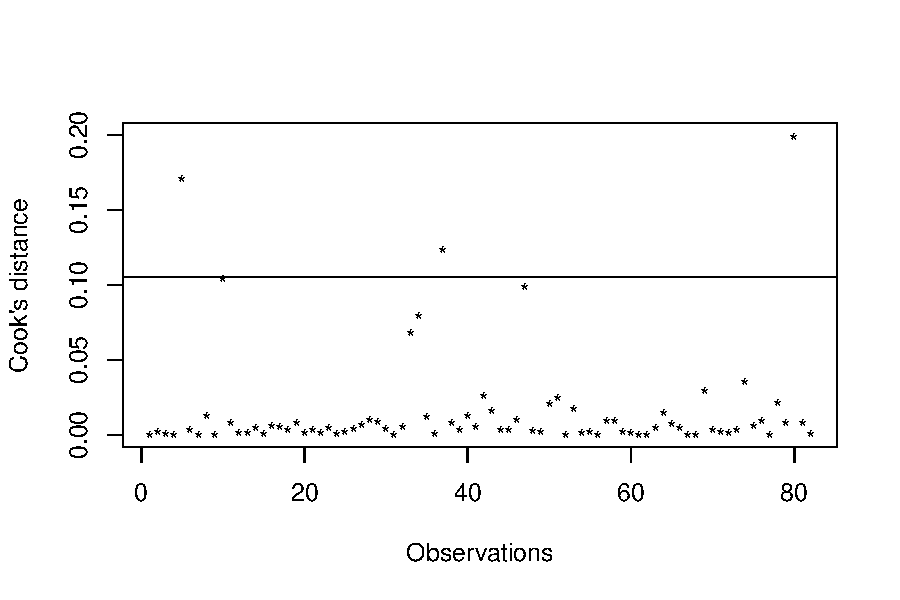
\includegraphics[width=3in]{cook.pdf}
}
\subfigure[Hat Values (leverage).\label{subfig:hats}]{
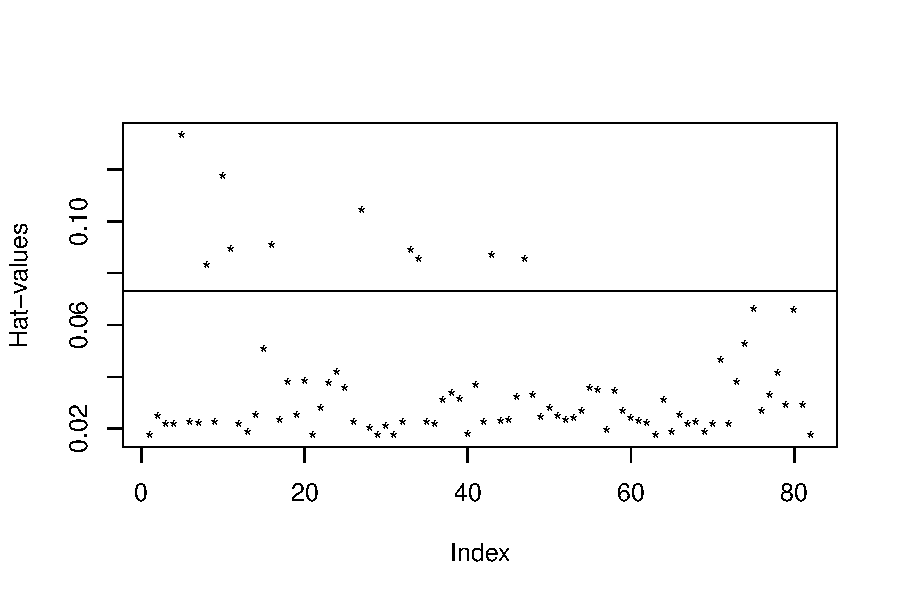
\includegraphics[width=3in]{hats.pdf}
}
\subfigure[Homoskedasticity.\label{subfig:fitted}]{
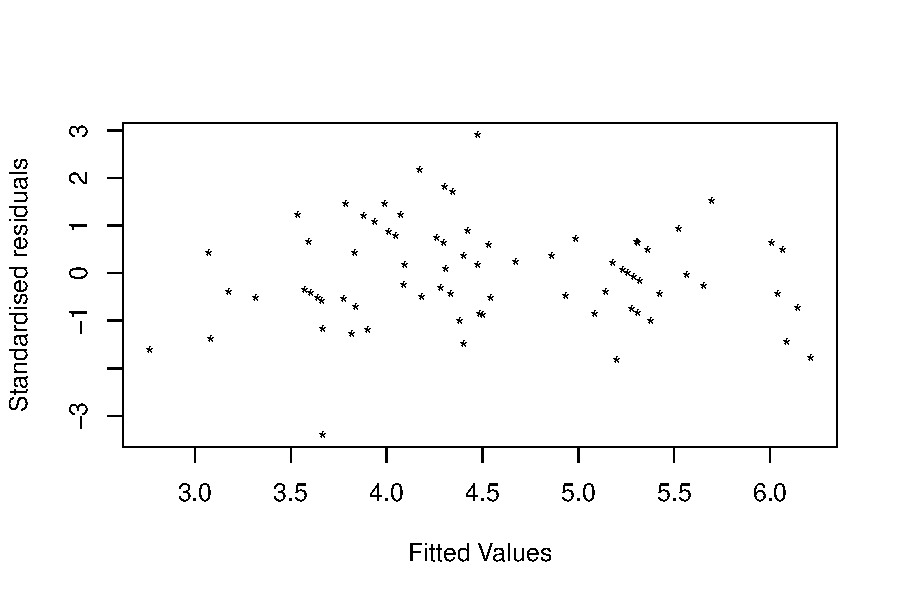
\includegraphics[width=3in]{fitted.pdf}
}
\subfigure[Q-Q normal plot.\label{subfig:qq}]{
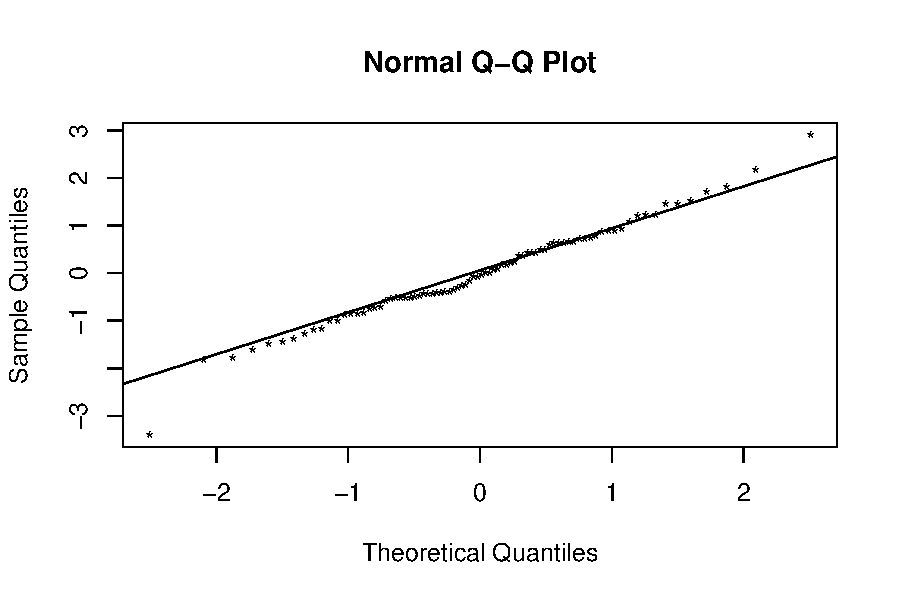
\includegraphics[width=3in]{qq.pdf}
}
\caption{Diagnostic plots for model $\frac{100}{City MPG} = \beta_0 + \beta_1Weight + \beta_2Cylinders + \epsilon.$}
\label{fig:diagnostics}
\end{figure}

We see no problem checking for homoskedasticity (Figure \ref{subfig:fitted}) and normality (Figure \ref{subfig:qq}). On the other hand Cook's distance plot (Figure \ref{subfig:cook}) and hat-values
plot (Figure \ref{subfig:hats}) have more points above the threshold than usual. First, no value
exceeds 0.20 on either graph then we might say we are still far from fitting the line exactly (hatvalue = 1.0). However, given the number of influence points we might want to look back in the
data set and examine source of those data points for further insight.
Second, the model we choose is really low dimensional, therefore we expect that the threshold being
so low\ldots that the original explanatory variables won't be absolutely be conformed to this subspace.

\section{Discussion and conclusions}
From our study on model selection and collinearity in the \emph{cars} dataset we have a few conclusions. One is that there is a trade-off between significance (in the p-value/AIC/BIC sense) and
variance inflation (VIF). It is not clear how to generalize this, but in our study the source of the
problem was that covariates with high linear dependence always ended up in the models with our most significant variables (e.g. \texttt{Wheelbase}) even if the latter are not specially significant.
Then, we acknowledge that what worked for us is manual scrutiny of the data. This means looking for those linear dependence
relationships ``by hand'' (Section \ref{sec:thedata}). Of course, this task is tedious and not very promising with the initial datasets. But, automatic model selection procedures like Forward/Backward methods do reduce the search space to find relevant models. We then focus on more evident associations between the covariates and hopefully traceback the problem
back to the source (with simple exploratory analysis for example).

Therefore, we see the value of the interplay between automatic procedures with human expertise. None of these parts is
perfect, but together as an iterative process they make up a much more coherent enterprise.

\appendix
\section{Appendix}
\begin{verbatim}
load('cars.RData')
require(car) 
library(xtable)

# the response y : 100 / City MPG
hundredOverMPG <- rep(100,82) / cars$CityMPG

# the variables
weights <- cars$Weight
HPOverWeight <- cars$Horsepower / cars$Weight

# Look if there is a correlation between our y
#and the variable we are going to use
pdf(file="ScatterWeights.pdf", width=6,height=4)
plot(weights, hundredOverMPG, xlab='Weights',
     ylab='Gallons per hundred city miles',pch='*')
dev.off()
pdf(file="ScatterPower.pdf", width=6,height=4)
plot(HPOverWeight, hundredOverMPG, xlab='HorsePowerPerWeight',
     ylab='Gallons per hundred city miles',pch='*')
dev.off()

# correlations
cor(weights, hundredOverMPG)#0.9007547
cor(HPOverWeight, hundredOverMPG)#0.5976514

# Fit first model in order: Y = b0 + X1*b1 + X2*b2
fit1 = lm(hundredOverMPG ~ weights + HPOverWeight)
fit1_w = lm(hundredOverMPG ~ weights)
# Fit second model in order: Y = b0 + X2*b2 + X1*b1
fit2 = lm(hundredOverMPG ~ HPOverWeight + weights)
fit2_hp = lm(hundredOverMPG ~ HPOverWeight)
# ANOVA tables
anova(fit1)
anova(fit1_w, fit1)
anova(fit2)
anova(fit2_hp, fit2)

# Scatterplots of variables that are strongly correlated
pairs(~Weight+FuelCapacity+Length+Wheelbase+Width+Uturn, data=cars)
cor(cars$Weight,cars$FuelCapacity)#0.9001302
cor(cars$FuelCapacity,cars$Wheelbase)#0.7934098
cor(cars$FuelCapacity,cars$Uturn)#0.6741421
cor(cars$FuelCapacity,cars$Width)#0.7717577
cor(cars$FuelCapacity,cars$Length)#0.794308

# ------------------- PART 2 : Model Selection --------------------

# Variables from 11 to 26 to fit a new model.
newData <- cars[ ,11:26]

FullFit <- lm(hundredOverMPG ~ ., data = newData)
summary(FullFit)
print(xtable(summary(FullFit)))
# Latex table
#summaryFullFit <- xtable(summary(FullFit))
#print(summaryFullFit)

# VIF of the full model
library(car)
vif(FullFit)
print(xtable(vif(FullFit)))
# ---Model Construction : Backward/Forward selection using AIC/BIC

# AIC, Backward
f1 <- lm(hundredOverMPG ~ ., data = newData)
f1.backward <- step(f1, direction = "backward")
summary(f1.backward)
vif(f1.backward)
# AIC, Forward
f2 <- lm(hundredOverMPG ~ 1, data = newData)
my.scope <- formula(data.frame(hundredOverMPG, newData))
f2.forward <- step(f2, scope = my.scope,
                   direction = "forward", data = newData)
summary(f2.forward)
vif(f2.forward)

# BIC, Backward
f3 <- lm(hundredOverMPG ~ ., data = newData)
# Fitting model using all the covariates
f3.backward <- step(f3, direction = "backward", k=log(nrow(newData)))
summary(f3.backward)
vif(f3.backward)
# BIC, Forward
f4 <- lm(hundredOverMPG ~ 1, data = newData)
# Fitting the model with only one varialbe, the 1 column
my.scope <- formula(data.frame(hundredOverMPG, newData))
f4.forward <- step(f4, scope = my.scope, direction = "forward",
                   data = newData, k=log(nrow(newData)))
summary(f4.forward)
vif(f4.forward)

# ----------------------------------------------------------------
# --Model without predictors showing a sign of multicollinearity--

#New regression without these variables
newData2 = cars[,-c(1,2,3,4,5,6,7,8,9,10,17,19,20,21,22)]
newFit <- lm(hundredOverMPG ~ ., data = newData2)
summary(newFit)
print(xtable(newFit))
# Latex table
#summaryNewFit <- xtable(summary(newFit))
#print(summaryNewFit)

# VIF of the full model
library(car)
vif(newFit)

# ------ Model Construction :
#Backward and Forward selection using AIC and BIC

# AIC, Backward
f1 <- lm(hundredOverMPG ~ ., data = newData2)
f1.backward <- step(f1, direction = "backward")
summary(f1.backward)
vif(f1.backward)
# AIC, Forward
f2 <- lm(hundredOverMPG ~ 1, data = newData2)
my.scope <- formula(data.frame(hundredOverMPG, newData2))
f2.forward <- step(f2, scope = my.scope,
                   direction = "forward", data = newData2)
summary(f2.forward)
vif(f2.forward)

# BIC, Backward
f3 <- lm(hundredOverMPG ~ ., data = newData2) 
# Fitting model using all the covariates
f3.backward <- step(f3, direction = "backward", k=log(nrow(newData2)))
summary(f3.backward)
vif(f3.backward)
# BIC, Forward
f4 <- lm(hundredOverMPG ~ 1, data = newData2) 
# Fitting the model with only one varialbe, the 1 column
my.scope <- formula(data.frame(hundredOverMPG, newData2))
f4.forward <- step(f4, scope = my.scope, direction = "forward",
                   data = newData2, k=log(nrow(newData2)))
summary(f4.forward)
vif(f4.forward)

# We see that we have two models, one with the BIC
#( backward and forward give the same model)
# and one with the AIC

# ------------- DIAGNOSTICS FOR THE TWO MODELS ------------
modelB <- f4.forward

# Plot fitted values against standardised residual
plot(modelB$fitted.values, rstandard(modelB), xlab="Fitted Values"
     , ylab="Standardised residuals")

# QQ plot
qqnorm(rstandard(modelB))
qqline(rstandard(modelB))

# Cook Distance
plot(cooks.distance(modelB), xlab='Observations', ylab="Cook's distance",
     ylim=c(0,0.2))
p <- dim(model.matrix(modelB))[2]
n <- dim(model.matrix(modelB))[1]
abline(8/(n-2*p),0)
plot(hatvalues(modelB), xlab = "Index", ylab="Hat-values")
abline(2*p/n,0)

\end{verbatim}

\newpage
\bibliography{Bibliographie}
\bibliographystyle{plain}

% Add the References to the table of contents.
\addcontentsline{toc}{section}{References}

\end{document}
